\chapter{Camera and object GUI main controls}
\minitoc  

 \section{Camera controls}
\subsection{Zoom}
There are three ways to modify the ``zoom" in ISE-MeshTools :


\begin{minipage}{0.7\textwidth}
\begin{itemize}
\item You may use the zoom roller laying in the lower part of the right panel of the main window.
\item	You may open the camera options window (viewing opt. $\rightarrow$  Camera $\rightarrow$ Camera options) and modify manually the ``Zoom" control.
\item	You may set manually the display scale (viewing opt $\rightarrow$ Camera $\rightarrow$ Set 100 pixels in mm)
\item	You may use the middle click mouse roll button (roll the wheel).
\end{itemize}
\end{minipage}    
\begin{minipage}{0.25\textwidth}\centering
  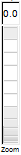
\includegraphics[scale=0.5]{images/Icons/zoom_01.png}
 \captionof{figure}{Zoom Roll}
 \end{minipage}    


When the option ``Adapt field of view depth" is active in the Rendering options window (Viewing opt.$\rightarrow$General rendering options $\rightarrow$ Depth of field of view panel), changing the zoom value will also modify the depth of the field of view (camera.far value) and the position of the clipping plane (camera.tz value). When the option ``Keep current field of view depth" is active, changing the zoom will not affect the camera.far and camera.tz values.

\subsection{Camera rotation around ``z" viewing axis}

\begin{minipage}{0.7\textwidth}
To do so, you may use the slider lying in the upper part of the right panel of the main window.
\end{minipage}    
\begin{minipage}{0.25\textwidth}\centering
  
\includegraphics[scale=0.5]{images/Icons/Rotation_z.png}
 \captionof{figure}{Camera ``z" rotation slider}
 \end{minipage}    



\subsection{Clipping plane}

\begin{minipage}{0.7\textwidth}
In some cases, you may need to displace the viewing clipping plane. To do so, use
the slider lying centrally in the right panel of the main window.\\
You can also modify the clipping plane manually by editing the ``Tz" control in
the camera options window (viewing opt. $\rightarrow$ Camera $\rightarrow$ Camera options).
The buttons 
\includegraphics[scale=0.7]{images/Icons/clipping_plane3.png} and 
\includegraphics[scale=0.7]{images/Icons/clipping_plane2.png} which lie just underneath the clipping plane slider (and
also in the camera option window) also permit to adjust / readjust the position of
the clipping plane at predefined positions :
\begin{itemize}
\item  
\includegraphics[scale=0.7]{images/Icons/clipping_plane3.png}: the clipping plane is placed at z = 0 (all objects having a z coordinate along
z viewing axis smaller than 0 are hidden).
\item	
\includegraphics[scale=0.7]{images/Icons/clipping_plane2.png} : the clipping plane is replaced at its original value : z= - camera.far / 2. This value permits to
view objects having positive and negative coordinates along z viewing axis.

\end{itemize}
\end{minipage}    
\begin{minipage}{0.25\textwidth}\centering
  
\includegraphics[scale=0.5]{images/Icons/clipping_plane.png}
 \captionof{figure}{Camera clipping plane slider}
 \end{minipage}   




\subsection{Camera orientation}
6 camera positions are predefined :\\

\includegraphics[scale=0.7]{images/pixmap/right2.png} view object from right side \\

\includegraphics[scale=0.7]{images/pixmap/left2.png} view object from left side\\

\includegraphics[scale=0.7]{images/pixmap/right2.png} view object from front side (default camera position)\\

\includegraphics[scale=0.7]{images/pixmap/front2.png} view object from back side\\

\includegraphics[scale=0.7]{images/pixmap/above2.png} view object from above\\

\includegraphics[scale=0.7]{images/pixmap/back2.png} view object from below\\

\subsection{Coordinate system orientation helper}
\begin{minipage}{0.7\textwidth}
Press 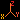
\includegraphics[scale=0.7]{images/pixmap/grid2.png} to show / hide the coordinate system orientation helper lying on the bottom left corner of the main 3D window. By default, the labels are defined
the following way:\\
+z axis : dorsal side\\
-z axis : ventral side\\
+y axis : left side\\
-y axis : right side\\
+x axis : proximal side\\
-x axis : distal side.\\
You may edit these labels depending on your preferences (for instance,
depending on the structure you are working with, you may need to set ``+y" to ``labial", and ``-y" to
``lateral"). To edit orientation labels, click on ``viewing opt. $\rightarrow$ Orientation labels."
\end{minipage}    
\begin{minipage}{0.3\textwidth}\centering
 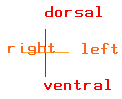
\includegraphics[scale=0.7]{images/GUI/Helper.png}
 \captionof{figure}{Orientation helper}
 \end{minipage}   

\subsection{Grid}
Press 
\includegraphics[scale=0.7]{images/pixmap/grid3.png} to show / hide the grid. Default grid size is 1 cm / square. Grid size can be edited manually
(viewing opt. $\rightarrow$ Grid size).
Switching between the 6 camera predefined positions defined above (
\includegraphics[scale=0.7]{images/pixmap/right2.png},
\includegraphics[scale=0.7]{images/pixmap/left2.png},
\includegraphics[scale=0.7]{images/pixmap/right2.png}, 
\includegraphics[scale=0.7]{images/pixmap/front2.png}, 
\includegraphics[scale=0.7]{images/pixmap/above2.png} and 
\includegraphics[scale=0.7]{images/pixmap/back2.png})will
affect the plane in which the grid is drawn.

\subsection{Lightning}
6 lightning orientations are predefined :\\

\includegraphics[scale=0.7]{images/pixmap/s_right_17.png}light from right viewing side\\

\includegraphics[scale=0.7]{images/pixmap/s_left_17.png}light from left viewing side\\

\includegraphics[scale=0.7]{images/pixmap/s_face_17.png}light from front viewing side\\

\includegraphics[scale=0.7]{images/pixmap/s_back_18.png}light from back viewing side\\

\includegraphics[scale=0.7]{images/pixmap/s_dessus_18.png}light from above\\

\includegraphics[scale=0.7]{images/pixmap/s_dessous_18.png}light from below\\

  \section{Object controls controls}
	As seen earlier, selected objects can be translated and rotated using the mouse left and middle buttons
(in landmark and camera selection modes, you also need to maintain ``CTRL" button pressed
while dragging the mouse to achieve rotation and translation of selected objects). Alternatively, you
may also use the following controls to accomplish rotation and translation of selected objects. Rotation
is performed around the global center of mass of all selected objects.

\subsection{Rotation around and translation along ``z" viewing axis}

\begin{minipage}{0.7\textwidth}
These controls are extremely useful, as there is no way to achieve rotation
around « z » viewing axis or translation along ``z" viewing axis using the
mouse. \\
To do so, use the slider and roller lying in the upper part of the left panel of the
main window.

\end{minipage}    
\begin{minipage}{0.25\textwidth}\centering
  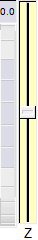
\includegraphics[scale=0.5]{images/Icons/x_rot.png}
 \captionof{figure}{Object ``z" rotation roller and slider}
 \end{minipage}    


\subsection{Rotation around ``x" and translation along ``y" viewing axes}

\begin{minipage}{0.7\textwidth}
To do so, use the slider and roller lying in the lower part of the left panel of the
main window.
\end{minipage}    
\begin{minipage}{0.25\textwidth}\centering
  \includegraphics[scale=0.5]{images/Icons/y_rot.png}
 \captionof{figure}{Object ``x" roller and ``y" slider}
 \end{minipage}   

\subsection{Rotation around ``y" and translation along ``x" viewing axes}


\begin{minipage}{0.5\textwidth}
To do so, use the slider and roller lying in the left part of the bottom panel of the
main window.
\end{minipage}    
\begin{minipage}{0.4\textwidth}\centering
  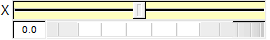
\includegraphics[scale=0.5]{images/Icons/z_rot.png}
 \captionof{figure}{Object ``y" roller and ``z" slider}
 \end{minipage}   

